\section{Experimental Results}\label{sec:performStudy}
We here present performance tests
to support our claims that our solution
is efficient and applicable in a real world
scenario. We have implemented a prototype of our solution, as well as
\hc \cite{pbsPaper} and \ff \cite{ffinder} for comparison.
For simplicity in comparing the two implementations,
$\Gamma$ contains granularities as a grid with uniform squares, 
where edge length $B(l)$ depends on level $l$.
We set $B(l)=L_0\cdot2^{-l}$ where $l$ is level and $L_0$ is the cell side
length at level 0. $L(l)=B(l)\sqrt{2}$ in this case.  


\subsection{Filtering and Unrestricted Vicinities}
The \vls ability to handle user vicinities of arbitrary shapes can also be
used to minimize the amount of granules needed to be sent to server. We
develop a road network filter(\rf) based on assumption that all users move on
the road network being interested in friends, falling in a circular
location-centered area.

When \rf is enabled, users use solid location-centered circle intersection
(black polygons in Fig. \ref{fig:ui_rf}b) with road segments as their
vicinities. An example of such vicinity type being rasterized (mapping user vicinity into
set of granules) is depicted in Fig. \ref{fig:ui_rf}b as dark cells. In order to
realistically simulate real roads with the \rf, especially with dense grids at
high levels, the road edges are represented as polygons. We
choose the width of polygons based on road classifications.



\begin{figure}
       \center
       \begin{tabular}{cc}	
			  \includegraphics[width=0.17\textwidth]{vl/images/incUpdDemo.pdf} &
	   		\includegraphics[width=0.17\textwidth]{vl/images/rn_dump5.pdf} \\	 
	   		\footnotesize Granules deletion and 				  &	\footnotesize Vicinity after rasterization \\
        \footnotesize insertion sets									& \\
           (a) & (b) \\
               
       \end{tabular}
       \caption{\iu and \rf optimizations}
  \label{fig:ui_rf}
\end{figure}


When \rf is used together with incremental updates (See sec. 
\ref{sec:optIncUpd}) the sets of granules, needed to be sent to server 
by user $u$ is further reduced by only considering the road segments within the
area of $U_{ts=0}$,$U_{ts=1}$ (see Fig \ref{fig:ui_rf}a.


\subsubsection{Data Generation}
The generator \cite{brinkhoff} was used to generate datasets based upon the
German city of Oldenburg. The datasets cover an area of $26915*23572$
$units^2$, corresponding to $14*12.26$ $km^2$, and they contain location
records for each user at each time stamp. The duration between two consecutive
timestamps is 1 minute and the average speed of the users is 52 km/h (i.e. 1670
units per time stamp).

\subsubsection{Test System Parameters}
\hc, \ff, and \vl share a number of settings which we,
unless otherwise stated, set to default values: the number of users is set to
50000; the number of timestamps is set to 40 (producing a workload
of 2 million location records); users are partitioned into disjoint
groups, each group containing 250 users. Within the same group, the
friend relationships between users form a complete graph.

Default cell size $L_0$ is 12800 units and the maximum level allowed by users,
denoted $L_{\epsilon}$ and $L_{max}$ for \ff and \vl respectively, is set to 6,
yielding cell side lengths of 200 units at this level. In the \vl, the vicinity
region is circular, and the default radius is 500, corresponding to 260 meters.

We consider two cases for \hc: minimum privacy and total privacy. For min.
privacy we set $G^{sp}$ and $G^{u}$ equal to 200 to mirror the same minimum user
location privacy as in \vl \& \ff. For maximum privacy we set $G^{sp}=80000$, to
force \hc to detect proximity in peer-to-peer mode, revealing no spatial
information to the server.

\subsubsection{Experiments}

\begin{figure*}[htb]
       \center
       \begin{tabular}{c c c c}			   
    \includegraphics[width=0.23\textwidth]{vl/images/lmax.pdf}&
    \includegraphics[width=0.23\textwidth]{vl/images/radiusIncOptimized.pdf} &
    \includegraphics[width=0.23\textwidth]{vl/images/lzcsR200u5-10.pdf}	&
    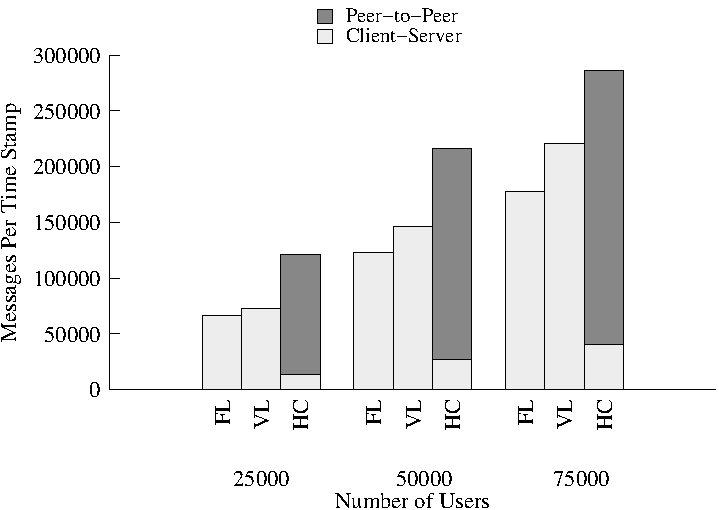
\includegraphics[width=0.23\textwidth]{vl/images/manyUsers.pdf} \\
          (a) & (b) & (c) & (d)
       \end{tabular}
  \caption{ 
   (a) Effect of increasing $L_{max}$.
   (b) Granules sent when increasing radius of vicinity.
   (c) Messages sent when increasing $L_0$, keeping $B(L_{max})$
       constant.
   (d) Server messages for one time stamp.  }
  \label{fig:lmax_Radi}
\end{figure*}

We will focus mainly on the performance parameter of messages and granules
since they are important parameters in real world usage and users will have
to pay for data when using \vl.

In Fig. \ref{fig:lmax_Radi}a we show the cost of increasing the precision of proximity detection.
We increase $L_{max}$, the number of possible levels users can shift
into. The experiment was run with no optimizations, with incremental
updates(\iuns), with road network filter(\rfns), and both road
network filter and incremental updates (\iu \& \rfns). 
At level 10 the \iu and \rf techniques respectively save a user 50\% and 80\% 
of the granules he would have to send with no optimization. When we combine \iu
and \rf we send less than 10\% of the granules sent by the unoptimized version
of \vl.

   
In Fig. \ref{fig:lmax_Radi}b we show the effect on number of granules sent when
increasing the radius of user's vicinity. When using \rf there is a significant
reduction which, as expected, is larger when the radius increases. This is
because there are more road segments to work on. The \iu optimization perform
well giving a linear increase in granules, as oppose to the quadratic increase
without optimization. The \rf and \iu combination performs excellent, reducing
the granule count even more. The amount of messages does not change for either
of the options.


We want to motivate what an optimal cell side length at level 0, the $L_0$,
might be. Note that changing $L_0$ gives the effect that there will be fewer
or no level shifts (but maybe more cell boundary crossings) in order to have the
same proximity detection precision. To this end we vary $L_0$ and $L_{max}$,
keeping $B(L_{max})=200$ and user's vicinity radius equal to 200 throughout the
tests (See Fig. \ref{fig:lmax_Radi}c). We compare against \ff with equivalent
precision, where setting of $\epsilon$ is equal to 200. We plot the
graph for 5 and 10 users in the system, setting all users in one group for each
test. 
We run \hc prototype with $\delta_A=200$ to demonstrate what a user would
pay in terms of messages, when a complete privacy or \vl-equivalent level of
minimum privacy is required. The graph shows results of \hc with minimum privacy
only. When maximum privacy is required numbers for 5/10 users are 8.2/14.88
messages. It is clear from Fig. \ref{fig:lmax_Radi}c that \vl performs better
than its competitors and that enabling of the levels allows to reduce amount of
client communication. The optimal $L_0$ for \vl or \ff is the lowest point on
the graphs in Fig. \ref{fig:lmax_Radi}c.



Figure \ref{fig:lmax_Radi}d show the total amount of messages sent by 25000,
50000, and 75000 users for one timestamp. Light bars correspond to client-server
messages, and dark bars to peer-to-peer messages of \hc with minimum privacy.
It is clear that \hc, even with minimum privacy (the communication is much
higher when complete privacy is required), incurs a higher amount of messages
compared to \vl or \ff due to expensive peer-to-peer communication. \vl
incurs reasonable amount of communication considering the the flexibility it
offers. Also note that \vl knows no users' spatial data unlike \hc, which
knows all users cloaking regions.
